% Source: Lecture22.pdf, pages 1-6. Title on the source: "Low-Density Series Expansions for Gases".
\lecture{22}
\subsection{Low-density series expansions for gases}

The van der Waals equation of state,
\begin{equation}
  \left[p + a\left(\frac NV\right)^2\right]\left[V-Nb\right] = N\kB T,
\end{equation}
also expressed in the equivalent forms in terms of the volume per particle $v = V/N$,
$\left(p + \frac{a}{v^2}\right)(v-b) = \kB T$, or $p = \frac{\kB T}{v-b} - \frac{a}{v^2}$, can also be written in terms of the
number density $\rho_n = \frac NV = \frac1v$; with $\beta = \frac{1}{\kB T}$:
\begin{equation}
  \beta p = \frac{1}{v-b} - \frac{\beta a}{v^2} = \frac{1}{\rho_n^{-1}-b} - \beta a\rho_n^2
  = \frac{\rho_n}{1-b\rho_n} - \beta a\rho_n^2,
\end{equation}
i.e.
\begin{equation}
  \boxed{\beta p = \rho_n\left[\frac{1}{1-b\rho_n} - \beta a\rho_n\right]}.
\end{equation}
Clearly, in the limit of a dilute gas, with $\rho_n\to 0$, this reduces to the ideal gas equation of state (EOS),
$\beta p = \rho_n$. Expanding the denominator, the vdW EOS has the form of an infinite series,
\begin{equation}
  \beta p = \rho_n\left[\sum_{j=0}^\infty(b\rho_n)^j - \beta a\rho_n\right]
          = \rho_n\left[\underbrace{1}_{\text{ideal gas EOS}} + \underbrace{\sum_{j=1}^\infty(b\rho_n)^j - \beta a\rho_n}_{\text{vdW corrections to ideal gas}}\right],
\end{equation}
with radius of convergence $|\rho_n| = \frac1b$, the position of the pole in $\frac{1}{1-b\rho_n}$.

More generally, one can describe the corrections to the ideal gas EOS via a Taylor series expansion in the number
density $\rho_n$:
\begin{equation}
  \beta p = \rho_n\left[1 + \sum_{\ell=1}^\infty B_{\ell+1}\rho_n^\ell\right]
\end{equation}
(since $B_{\ell+1}\rho_n^\ell$ is dimensionless, $\dim(B_{\ell+1}) = V^\ell$; $\dim(B_2) = V$, $\dim(B_3) = V^2$,
etc.). Since the expression in square brackets is an expansion around $\rho_n = 0$, this is a low-number-density
expansion. (Since the actual mass density $\rho\propto\rho_n$, this is equivalently a low-density expansion.) For
historical reasons, it is commonly called a ``virial expansion'':
\begin{equation}
  \beta p = \sum_{j=1}^\infty B_j\rho_n^j = \rho_n + \sum_{j=2}^\infty B_j\rho_n^j = \rho_n + B_2\rho_n^2 + B_3\rho_n^3 + \cdots,
\end{equation}
with $B_1 = 1$ to reproduce the ideal gas EOS, and the coefficient $B_j$ is called the $j$'th virial coefficient.
Thus, the $B_2\rho_n^2$ term is the leading correction to the ideal gas EOS. In contrast to the vdW EOS, which is a
2-parameter approximation, the virial expansion is a systematically improvable Taylor series expansion, analogous
to high-temperature and low-temperature expansions for spin models. For the vdW EOS,
\begin{equation}
  \beta p = \rho_n\left[1 + \sum_{\ell=1}^\infty(b\rho_n)^\ell - \beta a\rho_n\right]
          = \rho_n\left[1 + (b-\beta a)\rho_n + \sum_{\ell=2}^\infty(b\rho_n)^\ell\right]
\end{equation}
\begin{equation}
  \Rightarrow\quad B_2^{(\text{vdW})} = b-\beta a,\qquad B_j^{(\text{vdW})} = b^{j-1}\quad\text{for } j\ge 3 .
\end{equation}

In addition to being systematically improvable, the virial expansion can avoid unphysical aspects of the vdW EOS,
in particular, the region of $(p,V)$ where $(\partial p/\partial V)_T>0$, so that
$\kappa_T = -\frac1V\left(\frac{\partial V}{\partial p}\right)_T<0$.

The virial coefficients encode information about both the interactions between the gas particles and the
excluded-volume effect. This is evident in the $B_2$ coefficient for the vdW EOS, $B_2^{(\text{vdW})} = b-\beta a$.
At high temperature, $\beta\to 0$, the main effect is due to excluded volume, and $B_2^{(\text{vdW})}>0$
($\beta p>\rho_n$ to $\Order(\rho_n^2)$); as $T$ decreases, i.e.\ $\beta$ increases, eventually $b = \beta a$, so
$B_2^{(\text{vdW})} = 0$; and at low $T$, $B_2^{(\text{vdW})}<0$ ($\beta p<\rho_n$ to $\Order(\rho_n^2)$),
reflecting the importance of the interaction between the gas particles. This is also evident in the value of $T_c$
predicted by the vdW EOS, $\kB T_c = \frac{8a}{27b}\propto\frac ab$; the larger the excluded-volume effect is, the
lower one has to decrease the temperature to get condensation, while the larger the value of $a$, the higher the
temperature can be and still have condensation. The value $\beta = \frac ba$, i.e.\ $\kB T = \frac ab$, is the
``Boyle temperature'' for the vdW EOS; in general the Boyle temperature $T_{\text{Boyle}}$ is defined as the
temperature at which $B_2 = 0$, where the leading correction to the ideal gas (Boyle) law $\beta p = \rho_n$
vanishes.

\subsection{The second virial coefficient}

An illustrative calculation shows how the interaction between the gas particles (atoms or molecules) is embodied in
the virial coefficients. For this purpose, a standard approximation is to replace the repulsive term
$\left(\frac{r_0}{r}\right)^{12}$ in the Lennard-Jones 6--12 potential
$U = U_0\left[\left(\frac{r_0}{r}\right)^{12} - 2\left(\frac{r_0}{r}\right)^6\right]$, i.e.\
$U = 4U_0\left[\left(\frac\sigma r\right)^{12} - \left(\frac\sigma r\right)^6\right]$ where $r_0 = 2^{1/6}\sigma = 1.12\,\sigma$, with a hard cutoff in
$r$, so the model is called a ``hard sphere'' model:
\begin{equation}
  U(r) = \begin{cases} -U_0'\left(\frac\sigma r\right)^s & \text{for } r>\sigma\\ \infty & \text{for } r<\sigma .\end{cases}
\end{equation}
Here $r$, the distance between the centers of the hard spheres, cannot be smaller than $2r_{\text{sphere}}$, so
$U = \infty$ for $r<\sigma = 2r_{\text{sphere}}$. The weak attractive long-distance force is $\propto r^{-6}$ in
nature, but for the sake of generality, we let it be a general power $s\sim 6$.

\begin{diagram}
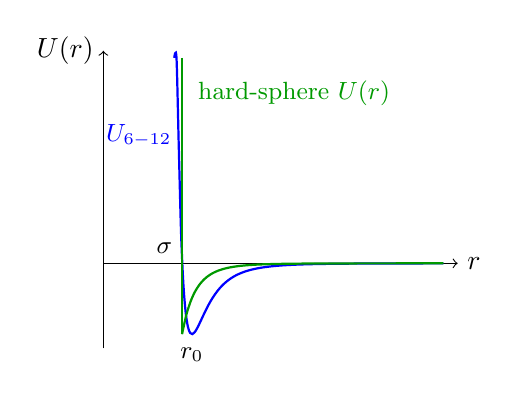
\begin{tikzpicture}[scale=0.9]
  \draw[->] (0,0) -- (5,0) node[right] {$r$}; \draw[->] (0,-1.2) -- (0,3) node[left] {$U(r)$};
  \draw[thick,blue,domain=1.0:4.8,samples=120,smooth] plot (\x,{max(-1.2,min(2.9,1.0*((1.25/\x)^12-2*(1.25/\x)^6)))});
  \draw[thick,green!60!black] (1.11,2.9) -- (1.11,-1.0);
  \draw[thick,green!60!black,domain=1.11:4.8,samples=60,smooth] plot (\x,{-1.0*(1.11/\x)^6});
  \node[above left,font=\small] at (1.11,0) {$\sigma$}; \node[below,font=\small] at (1.25,-1.05) {$r_0$};
  \node[blue,font=\small] at (0.5,1.8) {$U_{6\text{-}12}$};
  \node[green!60!black,font=\small,anchor=west] at (1.2,2.4) {hard-sphere $U(r)$};
\end{tikzpicture}
\diagramcaption{The Lennard-Jones 6--12 potential (blue) and the hard-sphere approximation (green).}
\end{diagram}

The partition function is
\begin{equation}
  Z = \frac{1}{N!}\int\left[\prod_{j=1}^N\frac{\dd^3r_j\,\dd^3p_j}{(2\pi\hbar)^3}\right]e^{-\beta\Ham},\qquad
  \Ham = \sum_{j=1}^N\frac{|\mathbf p_j|^2}{2m} + \sum_{j,k}U_{jk}
\end{equation}
(kinetic and potential terms). One can do the momentum part of the integration: for each of the 3 components
$(p_{jx},p_{jy},p_{jz})$ of $\mathbf p_j$, we use the Gaussian integration formula
$\int_{-\infty}^\infty\dd y\,e^{-\alpha y^2} = \sqrt{\pi/\alpha}$, so
$\int_{-\infty}^\infty\dd p_{jx}\exp\left[-\beta\frac{p_{jx}^2}{2m}\right] = \left[\frac{2m\pi}{\beta}\right]^{1/2}$ and hence
\begin{equation}
  \int\left[\prod_{j=1}^N\dd^3p_j\right]\exp\left[-\beta\sum_{j=1}^N\frac{|\mathbf p_j|^2}{2m}\right]
  = \left\{\left[\frac{2m\pi}{\beta}\right]^{1/2}\right\}^{3N},
\end{equation}
so write
\begin{equation}
  Z = \frac{1}{N!}\frac{1}{h^{3N}}\left(\frac{2\pi m}{\beta}\right)^{\frac{3N}{2}}
      \underbrace{\int\left[\prod_{i=1}^N\dd^3r_i\right]e^{-\beta\sum_{j,k}U_{jk}}}_{Z_U},
\end{equation}
where $Z_U$ encodes information on the interactions between the gas particles. The total potential energy is
\begin{equation}
  U = \sum_{j,k}U_{jk} = \binom N2u = \frac{N(N-1)}{2}u\simeq\frac{N^2}{2}u\quad\text{for } N\gg 1,
\end{equation}
where (lower-case) $u$ is the contribution to $U$ from each $j$--$k$ particle pair. For a given pair,
\begin{equation}
  \ev u = \frac{\int\dd^3r\,u\,e^{-\beta u}}{\int\dd^3r\,e^{-\beta u}} = -\pder{}{\beta}\ln\left[\int\dd^3r\,e^{-\beta u}\right].
\end{equation}
Since the interaction $u = u(r)$ decreases rapidly with increasing interparticle distance $r$, it is useful to
divide the integral as follows:
\begin{equation}
  \int\dd^3r\,e^{-\beta u} = \int\dd^3r\left[1 + (e^{-\beta u}-1)\right]
  = \underbrace{\int\dd^3r}_{V} + \underbrace{\int\dd^3r\,(e^{-\beta u}-1)}_{I}
  = V + I = V\left(1+\frac IV\right),
\end{equation}
so
\begin{align}
  u &= -\pder{}{\beta}\ln\left[\int\dd^3r\,e^{-\beta u}\right] = -\pder{}{\beta}\ln\left[V\left(1+\frac IV\right)\right]\nonumber\\
    &= -\underbrace{\pder{\ln V}{\beta}}_{0} - \pder{}{\beta}\ln\left[1+\frac IV\right]\simeq-\frac1V\pder I\beta,
\end{align}
since $I/V$ is small in the expansion. Now if $\beta = 0$, then
$Z_U = \int[\prod_{i=1}^N\dd^3r_i]e^{-\beta\sum_{jk}U_{jk}} = \int[\prod_{i=1}^N\dd^3r_i] = V^N$, so write
$\ln Z_U = N\ln V$ + a term involving interactions; use $U = -\partial\ln Z_U/\partial\beta$:
\begin{equation}
  \Rightarrow\ \ln Z_U = N\ln V + \int_0^\beta\frac{\partial\ln Z_U}{\partial\beta'}\dd\beta' = N\ln V - \int_0^\beta U(\beta')\dd\beta'.
\end{equation}
Recall $U\simeq\frac{N^2}{2}u\simeq-\frac{N^2}{2V}\pder I\beta$
\begin{equation}
  \Rightarrow\ \ln Z_U = N\ln V + \frac{N^2}{2V}\int_0^\beta\frac{\partial I(\beta')}{\partial\beta'}\dd\beta'
  = N\ln V + \frac{N^2}{2V}\left[I(\beta'=\beta) - \underbrace{I(\beta'=0)}_{=0}\right],
\end{equation}
so
\begin{equation}
  \ln Z_U = N\ln V + \frac{N^2}{2V}I(\beta);
\end{equation}
then the free energy is $A(T,V) = -\kB T\ln Z$: $\dd A(T,V) = -S\dd T - p\,\dd V$;
$p = -\left(\frac{\partial A}{\partial V}\right)_T = \kB T\left(\frac{\partial\ln Z}{\partial V}\right)_T$; now
$Z = \frac{1}{N!}\frac{1}{h^{3N}}\left(\frac{2\pi m}{\beta}\right)^{3N/2}Z_U$, so
\begin{equation}
  \left(\frac{\partial\ln Z}{\partial V}\right)_T = \left(\frac{\partial\ln Z_U}{\partial V}\right)_T = \frac NV - \frac{N^2}{2V^2}I,
\end{equation}
so
\begin{equation}
  \beta p = \left(\frac{\partial\ln Z}{\partial V}\right)_T = \frac NV - \frac12\left(\frac NV\right)^2I = \rho_n - \frac I2\rho_n^2;
\end{equation}
equating this to the leading terms in the virial expansion, $\beta p = \rho_n + B_2\rho_n^2 + \ldots$, we have
\begin{equation}
  \boxed{B_2 = -\frac12I = -\frac12\int\dd^3r\,(e^{-\beta u}-1)}.
\end{equation}
Now, in spherical coordinates,
\begin{equation}
  \int\dd^3r = \int r^2\dd r\int\dd\Omega = \int r^2\dd r\underbrace{\int_0^\pi\sin\theta\,\dd\theta\int_0^{2\pi}\dd\phi}_{4\pi}
  = 4\pi\int r^2\dd r
\end{equation}
for an integrand depending only on $r = |\mathbf r|$. So
\begin{equation}
  \boxed{B_2 = -2\pi\int(e^{-\beta u}-1)r^2\dd r}.
\end{equation}
The fact that $\dim(B_2)$ = volume is in accord with the general $\dim(B_{\ell+1}) = V^\ell$.

As noted above for $B_2^{(\text{vdW})} = b-\beta a$, and true more generally, at high temperature, i.e.\ small $\beta$,
the gas particles are not strongly affected by the attractive interaction, so $B_2>0$, and so, with
$\beta p = \rho_n[1+B_2\rho_n+\ldots]$, the pressure is slightly larger than for an ideal gas. At low temperature,
$\kB T\sim U_0$, the attractive interaction is important, so $B_2<0$ and the pressure is less than for an ideal gas.

\subsubsection*{Hard-sphere potential}

Now carry out an explicit calculation of $B_2$ for the hard-sphere potential
\begin{equation}
  U(r) = \begin{cases}-U_0'\left(\frac\sigma r\right)^s & \text{for } r>\sigma\quad\text{(long-distance attraction)}\\
                      \infty & \text{for } r<\sigma\quad\text{(hard-sphere term)}:\end{cases}
\end{equation}
$B_2 = -2\pi\int_0^\infty(e^{-\beta U}-1)r^2\dd r$; here, $-\beta U = +\beta U_0'\left(\frac\sigma r\right)^s = \beta U_0'\xi^{-s}$ for
$\xi>1$. Use the dimensionless variable $\xi = r/\sigma$, so
$B_2 = -2\pi\sigma^3\int_0^\infty(e^{-\beta U}-1)\xi^2\dd\xi$, and
\begin{equation}
  \int_0^\infty(e^{-\beta U}-1)\xi^2\dd\xi
  = \underbrace{\int_0^1(e^{-\infty}-1)\xi^2\dd\xi}_{-\frac13} + \int_1^\infty\left(e^{\beta U_0'\xi^{-s}}-1\right)\xi^2\dd\xi .
\end{equation}
To evaluate the second integral, use the Taylor series expansion $e^x = \sum_{n=0}^\infty\frac{x^n}{n!}$:
\begin{align}
  \int_1^\infty\left(e^{\beta U_0'\xi^{-s}}-1\right)\xi^2\dd\xi
  &= \int_1^\infty\dd\xi\Bigl[\underbrace{(1-1)}_{0}\xi^2 + \beta U_0'\xi^{-s+2} + \frac{1}{2!}(\beta U_0')^2\xi^{-2s+2}\nonumber\\
  &\qquad\qquad + \frac{1}{3!}(\beta U_0')^3\xi^{-3s+2} + \cdots\Bigr]\nonumber\\
  &= \left.(\beta U_0')\frac{\xi^{3-s}}{3-s}\right|_1^\infty + \left.\frac12(\beta U_0')^2\frac{\xi^{3-2s}}{3-2s}\right|_1^\infty + \cdots\nonumber\\
  &= -\frac{(\beta U_0')}{3-s} - \frac{(\beta U_0')^2}{2(3-2s)} + \cdots
\end{align}
(the evaluation at $\xi = \infty$ gives 0 because $s\sim 6$, so $3-s<0$, $3-2s<0$, etc.), so
\begin{equation}
  B_2 = -2\pi\sigma^3\left[-\frac13 - \frac{\beta U_0'}{3-s} - \frac{(\beta U_0')^2}{2(3-2s)} - \cdots\right],
\end{equation}
i.e.
\begin{equation}
  B_2 = \frac{2\pi\sigma^3}{3}\left[1 + \frac{3\beta U_0'}{3-s} + \frac{3(\beta U_0')^2}{2(3-2s)} + \cdots\right].
\end{equation}
Substituting the physical value $s = 6$:
\begin{equation}
  B_2 = \frac{2\pi\sigma^3}{3}\left[1 - (\beta U_0') - \frac{(\beta U_0')^2}{6} - \cdots\right].
\end{equation}
The first two terms have the same form as $B_2^{(\text{vdW})} = b-\beta a$ with the identifications
\begin{equation}
  b = \frac{2\pi\sigma^3}{3}\qquad\text{and}\qquad a = \left(\frac{2\pi\sigma^3}{3}\right)U_0' .
\end{equation}
See the graphs of determinations of $B_2$ from fits to data for several gases uploaded to BrightSpace (in the same
set as the vdW isotherm curves).

\subsection{The Clausius--Clapeyron equation}

Let us consider the liquid--gas phase coexistence curve (see the phase diagram in Figure~\ref{fig:pT}). At a given $p$ and $T$, crossing this curve from liquid to gas entails a discontinuous change in $V$
and also $S$ (entropy). The fact that the two phases are in equilibrium means that they have the same value of the
Gibbs free energy $G(T,p)$. Denote the gas phase as 2 and the liquid phase as 1. Recall
$\dd G = -S\dd T + V\dd p$; $\left(\frac{\partial G}{\partial T}\right)_p = -S$; $\left(\frac{\partial G}{\partial p}\right)_T = V$. So
$G_1 = G_2$ at any point along the liquid--gas coexistence curve. So $\dd G_1 = \dd G_2$:
\begin{equation}
  -S_1\dd T + V_1\dd p = -S_2\dd T + V_2\dd p\ \Rightarrow\ (S_2-S_1)\dd T = (V_2-V_1)\dd p;
\end{equation}
denote $\Delta S = S_2-S_1$, $\Delta V = V_2-V_1 = V_g-V_\ell\simeq V_g$ since $V_g\gg V_\ell$. Then
\begin{equation}
  \frac{\Delta S}{\Delta V} = \frac{\dd p}{\dd T}.
\end{equation}
Recall the relation of the latent heat $L_v$ of vaporization to the entropy change at temperature $T$:
$\Delta S = \frac{L_v}{T}$ for vaporization ($N = nN_A$; $n$ = \# moles). Then
\begin{equation}
  \frac{L_v}{T\Delta V}\simeq\frac{L_v}{TV_g} = \frac{\dd p}{\dd T}.
\end{equation}
Using the approximation that the ideal gas EOS describes the vapor at this $(p,T)$ point, i.e.\
$pV_g = N\kB T = nRT$, $\frac{1}{V_g} = \frac{p}{nRT}$, so
\begin{equation}
  \frac{L_v}{TV_g} = \frac{pL_v}{nRT^2} = \frac{\dd p}{\dd T}\ \Rightarrow\ \frac{L_v\dd T}{nRT^2} = \frac{\dd p}{p};
\end{equation}
here $L_v/n$ is the latent heat of vaporization per mole, denoted $L$. Integrating:
\begin{equation}
  \int\frac{\dd p}{p} = \frac LR\int\frac{\dd T}{T^2}\ \Rightarrow\ \ln p = -\frac{L}{RT} + \text{const.},\qquad
  \boxed{p = c\,e^{-\frac{L}{RT}},\ c = \text{const.}}
\end{equation}
Normalize by dividing by $p$ at a reference temperature $T_0$, $p_0 = c\,e^{-\frac{L}{RT_0}}$:
\begin{equation}
  \boxed{p = p_0\exp\left[-\frac LR\left(\frac1T-\frac{1}{T_0}\right)\right]}\qquad\text{(Clausius--Clapeyron equation for vapor pressure)}.
\end{equation}
This shows that $p$ is a rapidly increasing function of $T$, given the exponential dependence.

Some values of the molar latent heat of vaporization for some substances:
\begin{center}
\begin{tabular}{lc}
  substance & $L$\\ \hline
  N$_2$ & 5.57 kJ/mole\\
  O$_2$ & 6.82 kJ/mole\\
  H$_2$O & 40.7 kJ/mole\\
  Ne & 1.73 kJ/mole\\
  Ar & 6.45 kJ/mole
\end{tabular}
\end{center}
The fact that $L$ is much larger for H$_2$O than for the other substances is a consequence of the nonzero electric
dipole moment of H$_2$O; the others have zero (permanent) electric moment, as is obvious from symmetry.
